\chapter{Implémentation} \label{ch:implementation}

Le modèle se construit sur différents niveaux d’abstractions. L'exécution d'une simulation s'effectue en plusieurs étapes, du plus général au plus détaillé.

\section{Main}

Le main est la structure du plus haut niveau du modèle est sert d'interface pour l'utilisateur. A ce niveau, il est possible d'instancier plusieurs simulations avec des paramètres choisis. L'instanciation d'une simulations se fait de la manière suivante :

\begin{minted}
  [
  frame=lines,
  framesep=2mm,
  baselinestretch=1.2,
  bgcolor=LightGray,
  fontsize=\footnotesize,
  linenos
  ]
  {c++}
  threads.push_back(std::thread(thread_function, "./path_exemple"));
\end{minted}

Le programme utilise des threads afin de gagner en performances. Etant donné que les simulations sont difficilement parallélisables nous pouvons uniquement lancer plusieurs simulations simultanément. Une variable de précompilation dans le main définit le nombre de thread alloué au programme.

\begin{minted}
  [
  frame=lines,
  framesep=2mm,
  baselinestretch=1.2,
  bgcolor=LightGray,
  fontsize=\footnotesize,
  linenos
  ]
  {c++}
  #define NB_THREADS 8
\end{minted}

Cette valeur signifie que $8$ simulations peuvent être exécutée simultanément. Définissez cette valeur en fonction des ressources disponsibles.\\

Une simulation nécessite un chemin ou les informations seront lues et stockées. Afin de pouvoir exécuter une simulation il est nécessaire d'y ajouter un fichier de configuration contenant les paramètres de la simulation. Dans l'exemple, le dossier "path\_exemple" est accédé depuis la racine du projet et doit contenir le fichier de configuration de la simulation.\\

Le chemin vers le dossier est la racine de la simulation. Le fichier de configuration dans le dossier de la simulation doit avoir le nom suivant : \textbf{config.txt}.  A la fin de la simulation, le programme écrit les résultats dans un sous-dossier nommé "data\_csv". Les résultats sont des fichiers CSV contenant des informations sur la simulation.\\

Un ficher de configuration est un ficher texte contenant des lignes formées de mots clefs accompagnée de leur valeur. Un analyseur syntaxique parse le fichier puis les tokens sont analysés par un analyseur lexical qui s'occupe d'assigner les variables du modèles avec les valeurs lues dans le fichier de configuration.\\ 

La syntaxe du fichier de configuration doit être respectée. Les valeurs peuvent être modifiées par contre les noms doivent être identiques. L'analyseur lexicale n'est pas sensible aux espaces insérés entre les noms, le "=" ainsi que les valeurs.

\begin{minted}
[
frame=lines,
framesep=2mm,
baselinestretch=1.2,
bgcolor=LightGray,
fontsize=\footnotesize,
linenos
]
{c++}
TAILLE_SYSTEME = 894
NOMBRE_INDIVIDUS = 100000
ITERATIONS = 150
RERUN_LIMIT = 1000
FAIL_SEUIL = 10
GENOME_INIT_I = 0
GENOME_DIVERSITY_I = 0
GENOME_INIT_AP = 0
VITESSE_MUTATIONS_AP = 0
CHARGE_VIRALE = 1
PARAMETRE_FONCTION = 1
CELLULE_AP = 0
SURVIE_AP = 0
NOMBRE_MOUVEMENT = 1
PERFECT_MIX = false
TEMPS_AVANT_IMMUNITE = 1
IMMUNITE_MECANISME = false
RESISTANCE_MECANISME = false
\end{minted}

Voici la structure d'un fichier de configuration. Chaque ligne est composée d'un paramètre avec une valeur associée. 

\section{Initialisation}

La phase d'initialisation prépare le système pour une simulation. La première étape est de lire le fichier de configuration et d'assigner les valeurs lues aux variables de la simulation. Ensuite il faut allouer de la mémoire pour tous les objets du système. La simulation ainsi que les individus et les agents pathogènes sont des objets. Le nombre d'individus du système est déterminé par le paramètre {\small "NOMBRE\_INDIVIDUS"} et chaque individu est pointé par un pointeur appartenant à une liste. Cette liste est de taille fixe et contient tous les individus du système. Contrairement aux individus, les objets agents pathogènes ne sont pas contenus dans une liste fixe à cause de leur nombre pouvant changer. En effet, un agent pathogène est un objet à part entière si et seulement s'il contamine une cellule. Nous utilisons donc une liste doublement chaînée pour stocker ces objets. Cette structure permet de supprimer un élément au milieu de la liste sans créer de trou.\\ 

Le paramètre {\small "TAILLE\_SYSTEME"} nous indique la taille de la grille. Deux grilles sont instanciées comme des matrices de pointeurs pouvant pointer sur des objets. Une grille est dédiée à pointer sur les individus et une autre sur les agents pathogènes. Il est nécessaire d'utiliser deux grilles car il se peut que un individu et un agent pathogène se retrouvent sur la même cellule.\\

\begin{figure}[h]
\centering
\captionsetup{justification=centering}
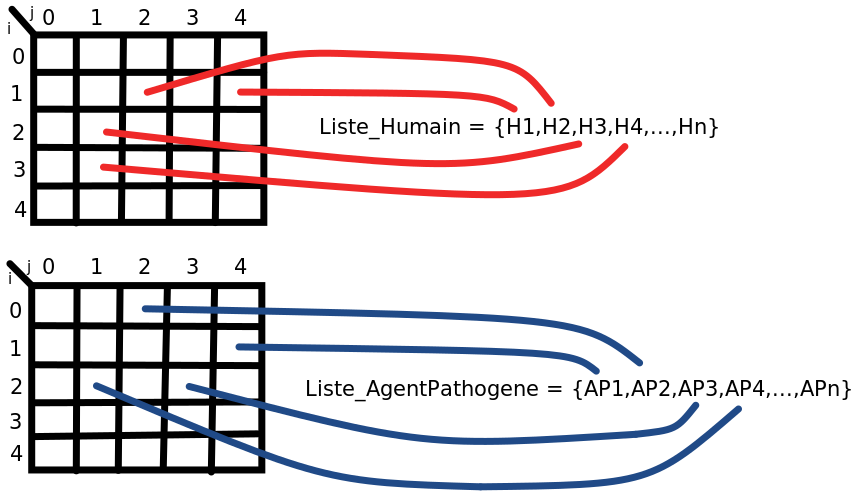
\includegraphics[scale=0.4]{Images/MatricesPointeurs.png}
\caption[Matrices de pointeurs]{L'espace est représenté par deux matrices de pointeurs de la taille du système. Chacune de ces matrices pointe exclusivement sur un type d'acteurs.}
\end{figure}

Après avoir créé les structures de données il faut générer les génomes des individus. Le génome initial de référence est donnée par le paramètre {\small "GENOME\_INIT\_I"}. Ce dernier sert de base pour la génération des génomes des individus. Le paramètre {\small "GENOME\_DIVERSITY\_I"} détermine le niveau de déviation par rapport aux génome de référence. Par conséquent, pour attribuer des génomes aux individus on part du génome de référence et modifions aléatoirement un nombre de bits déterminé par le paramètre {\small "GENOME\_DIVERSITY\_I"}. Par exemple, avec {\small GENOME\_DIVERSITY\_I} = 1, tous les individus auront le génome de référence avec un bits choisi aléatoirement dans la séquence qui sera complémenté. Ce mécanisme permet d'obtenir des génomes avec un certain degré de proximité à une certaine valeur choisie. Le génome de l'unique agent pathogène initial est défini par {\small "GENOME\_INIT\_AP"}.\\

L'étape suivante est de disposer tous les individus sur la grille et ceci aléatoirement. Finalement il faut contaminer un premier individu avec le pathogène initial. 

\section{Exécution de la simulation}

Une grande majorité du travail de la simulation s'effectue à cette étape. Cette phase se répète un nombre de fois équivalent à la valeur du paramètre {\small "ITERATIONS"}. Chaque itération sert à actualiser, à un moment donné le système en entier.

\subsubsection{Permutation}

La première étape est la construction d'une permutation des indices de la liste contenant les individus. Pour que le système soit aléatoire il est important de ne pas actualiser tous les individus dans le même ordre à chaque itération. C'est la raison pour laquelle nous permutons les indices de la liste des individus à chaque itération et la parcourons en suivant les indices permutés. Ceci permet d'actualiser tous les individus du système dans un ordre aléatoire.

\subsubsection{Agents pathogènes}

Vient ensuite le phase de mise à jour des agents pathogènes contaminant des cellules. Ces derniers sont détachés des individus et sont donc des objets à part entière. L'actualisation de ces agents pathogène s'effectue en une seule étape. Nous parcourons tous les agents pathogènes contaminant des cellules (l'ordre ici n'est pas important) et déterminons si les pathogènes survivent à cette itération. La probabilité de survie d'un tel agent pathogène est déterminé par le paramètre {\small "SURVIE\_AP"}. Ce facteur donne la probabilité qu'un agent pathogène contaminant une cellule survive à cette itération.

\subsubsection{Individus}

L'étape d'actualisation et de déplacement des individus est l'étape la plus coûteuse en temps. L'actualisation d'un individu se fait en deux étapes. La première étape consiste à calculer les interactions et mettre à jour les états et la seconde est d'effectuer un ou plusieurs déplacements.\\

La première chose à faire lorsque nous souhaitons actualiser un individu est de regarder si cet individu est contaminé. Si l'individu est déjà contaminé il est inutile de calculer les interactions avec ses voisins étant donnée qu'il est hôte d'un pathogène. Il nous reste donc à actualiser son état. Dans cette situation, notre individu n'a que trois issues. La première est d'être naturellement résistant au pathogène. La seconde est de s'immuniser au pathogène et la troisième est de conserver le pathogène.\\

Le paramètre booléen {\small "IMMUNITE\_MECANISME"} du modèle détermine si le mécanisme d'immunisation est actif ou non. Il en est de même pour le paramètre booléen {\small "RESISTANCE\_MECANISME"}. Désactiver ces mécaniques permet de simuler des systèmes ou l'immunisation est impossible. Il est aussi possible de déterminer le seuil temporelle différenciant la résistance naturelle de l'immunisation avec le paramètre {\small "TEMPS\_AVANT\_IMMUNITE"}. C'est-à-dire que cette variable détermine le temps minimal nécessaire pour que le rejet du pathogène soit considéré comme immunité.\\

Pour déterminer si un individu contaminé rejette ou non son agent pathogène à une certaine itération, nous utilisons une fonction calculant la compatibilité entre le pathogène et l'individu. La première étape pour calculer la compatibilité entre deux organismes est d'évaluer la distance de Hamming entre les deux séquences de génomes. L'entier résultant doit ensuite être converti en probabilité. La conversion s'effectue par une fonction dont une variable est définie par le paramètre du modèle {\small "PARAMETRE\_FONCTION"}.\\
$$
f(d) = \frac{d^{PARAMETRE\_FONCTION}}{32^{PARAMETRE\_FONCTION}} = (\frac{d}{32})^{PARAMETRE\_FONCTION}
$$
Le paramètre $d$ est la distance de Hamming entre les deux génomes des acteurs. Cette fonction traduit la distance de Hamming en une probabilité car $d$ ne peut varier que entre $[0,32]$.

\begin{figure}[h]
  \centering
    \captionsetup{justification=centering}
  \begin{minipage}[b]{0.4\textwidth}
    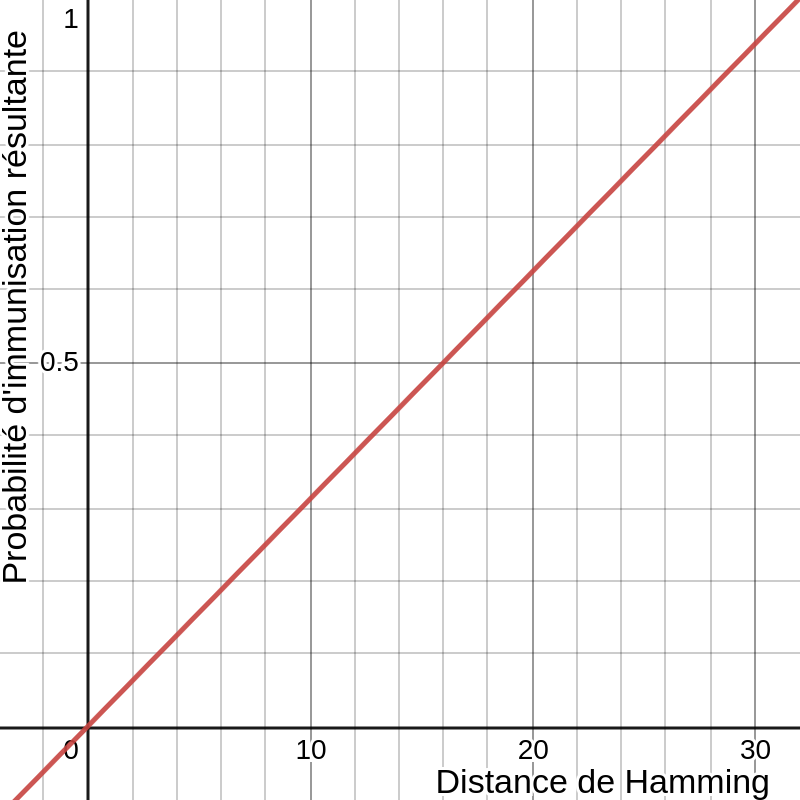
\includegraphics[width=\textwidth]{Images/fonction_1.png}
    \caption[Fonction de converstion en probabilité (facteur 1)]{Fonction de conversion de la distance de Hamming en probabilité avec {\small PARAMETRE\_FONCTION} = $1$}
  \end{minipage}
  \hfill
  \begin{minipage}[b]{0.4\textwidth}
    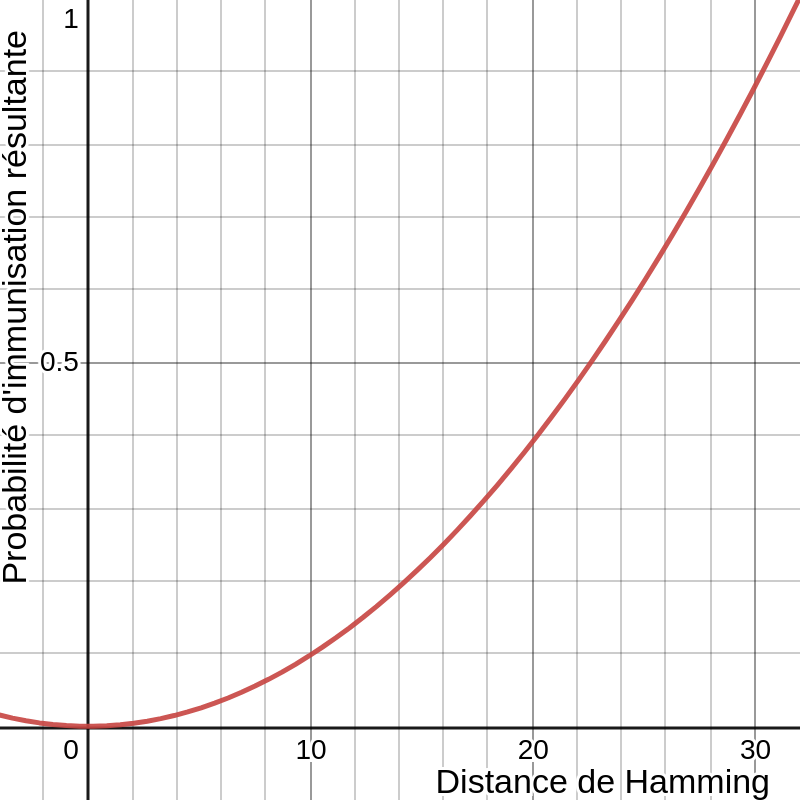
\includegraphics[width=\textwidth]{Images/fonction_2.png}
    \caption[Fonction de converstion en probabilité (facteur 2)]{Fonction de conversion de la distance de Hamming en probabilité avec {\small PARAMETRE\_FONCTION} = $2$}
  \end{minipage}
\end{figure}

\begin{figure}[h]
  \centering
    \captionsetup{justification=centering}
  \begin{minipage}[b]{0.4\textwidth}
    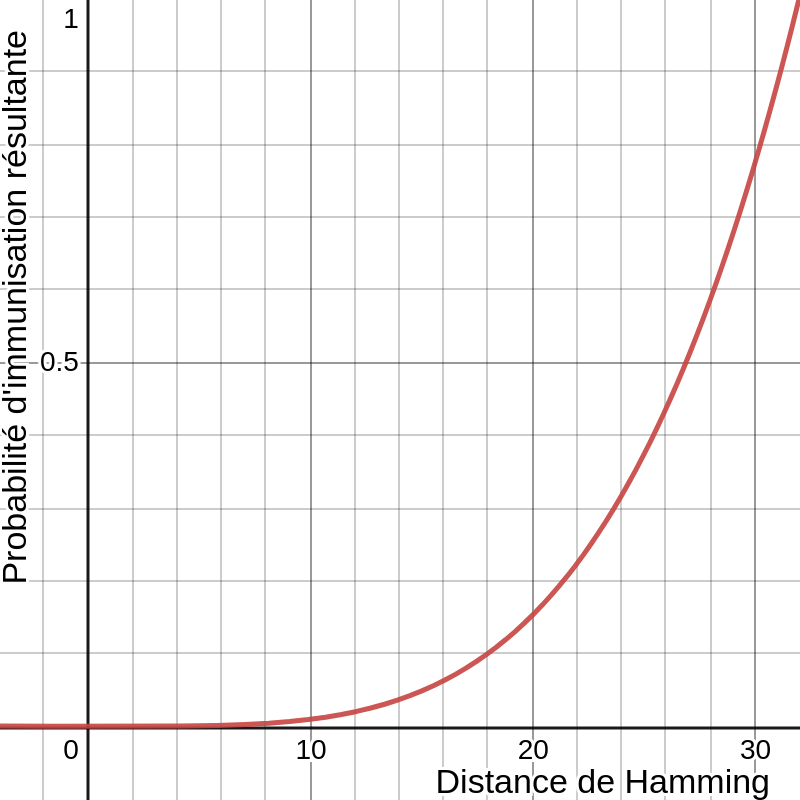
\includegraphics[width=\textwidth]{Images/fonction_4.png}
    \caption[Fonction de converstion en probabilité (facteur 4)]{Fonction de conversion de la distance de Hamming en probabilité avec {\small PARAMETRE\_FONCTION} = $4$}
  \end{minipage}
  \hfill
  \begin{minipage}[b]{0.4\textwidth}
    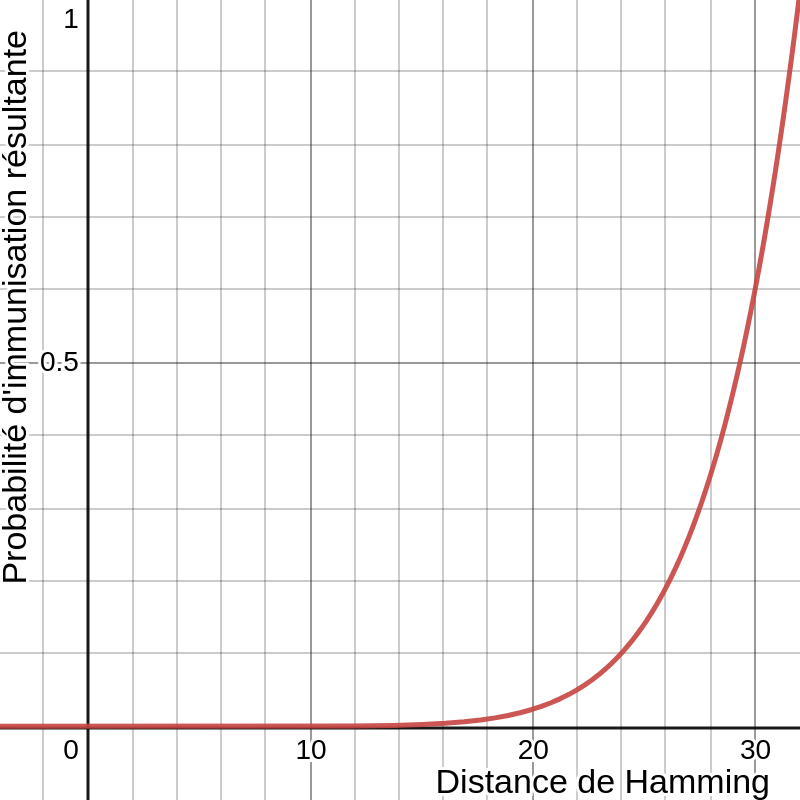
\includegraphics[width=\textwidth]{Images/fonction_8.png}
    \caption[Fonction de converstion en probabilité (facteur 8)]{Fonction de conversion de la distance de Hamming en probabilité avec {\small PARAMETRE\_FONCTION} = $8$}
  \end{minipage}
\end{figure}

Les $4$ fonctions sont bornées entre $[0,1]$. L'image en une abscisse représente la probabilité de rejetter l'agent pathogène en fonction de la distance de Hamming. Le paramètre de fonction permet de modifier l'allure de la courbe sans modifier les bornes. Une petite valeur de {\small "PARAMETRE\_FONCTION"} traduit de grandes probabilités d'éliminer l'agent pathogène et inversement une grande valeur du paramètre traduit en de faibles probabilités d'éliminer le pathogène.\\

Comme expliqué ci-dessus, à chaque itération, chaque individu contaminé a une chance de se débarrasser de son pathogène. Si l'individu contaminé n'y parvient pas, alors le pathogène a la possibiliter de muter. Le facteur de mutation de la simulation est donné par le paramètre {\small "VITESSE\_MUTATIONS\_AP"}. Ce paramètre borné entre $[0,1]$ détermine la probabilité qu'a un pathogène de muter dans un individu. En cas de mutation, un agent pathogène complémente aléatoirement un seul bit de sa séquence de génome.\\

Le processus de mise à jour pour les individus non contaminés est bien différent. Ces derniers n'intègrent pas de pathogène par conséquent nous nous intéressons qu'aux interactions avec les autres acteurs. Un individu sain est soumis à deux types d'interactions, la première est l'interaction avec des agents pathogènes contaminant des cellules de la grille et la seconde est l’interaction avec des individus dans le voisinage.\\

Les deux types d'interactions suivent la même méthodologie. La première étape de toutes interactions est donné par le paramètre {\small "CHARGE\_VIRALE"}. Ce paramètre borné entre $[0,1]$ détermine la probabilité qu'une interaction se produise entre deux acteurs en contact. La deuxième étape est la vérification des immunités. En effet, si l'individu est déjà immunisé au pathogène le contaminant, rien ne se produit. Sans protection l'individu est inévitablement contaminé par le pathogène.\\

La phase de déplacement se produit après la phase de mise à jour. A chaque itération un individu peut se déplacer un nombre de fois égal au paramètre {\small "NOMBRE\_MOUVEMENT"}. Le choix de la direction du déplacement est déterminé avant la vérification des cellules disponibles. En cas d'échec de déplacement dû à la non disponibilité de la cellule destination, le mouvement non effectué est tout de même comptabilisé. Cela signifie que si le paramètre de mouvement est défini à $10$, les individus se déplacent à chaque itération d'un nombre de cellules variant entre $[0,10]$ en fonction de la disponibilité.\\

Un individu contaminé se déplaçant a une chance de contaminer l'espace qu'il quitte. La probabilité de réaliser cet événement est donné par le paramètre {\small "CELLULE\_AP"} borné de $[0,1]$. En cas de contamination de cellule un nouvel objet agent pathogène est créé et porte le génome du pathogène de l'individu contaminé. 

\subsubsection{Mesures}

L'étape finale est la prise de mesures lors de la simulation, le traitement des données et l'écriture dans les fichier CSV. Les données récoltées sont le nombre de contaminés, le nombre d'agents pathogènes différents, le nombre d'individus ayant au moins une immunité ainsi que quelques autres informations relative à la simulation. Faire des mesures et analyses pendant la simulation nous évite de devoir sauvegarder toutes les données.\\

\section{Fermeture}

La phase de fermeture de la simulation effectue deux actions. La première est de fermer tous les fichier CSV et la seconde est de libérer tous les espaces mémoires alloués par la simulation.